	
	This thesis investigates models for gaining customer insights using graph
	machine learning. Graph machine learning is a current frontier in machine 
	learning and has many successful applications in many areas such as recently 
	shown by the success of AlphaFold \citep{senior2020improved}. AlphaFold made 
	a breakthrough for predicting protein structures where they made use of the 
	observation that a folded protein can be considered as a spatial graph 
	\citep{AlphaFoldTeam2020}. More generally, there are a vast range of 
	applications for graph machine learning in the fields of natural science, 
	social science and many more as shown by the excellent overview given by 
	\cite{zhou2020graph}. Graphs are especially useful as they allow for the 
	consideration of relationships between observations. Graph machine learning 
	has for that reason become a promising field as it allows for the use of
	richer data. This thesis will focus on graph machine learning for the
	purpose of customer classification. In particular, it is investigated to
	what extent semi-synthetic graphs can be used for graph machine learning.
	To provide a better overview as to how this topic relates to business \& 
	economics related fields such as gaining customer insights, some motivating
	examples are provided in the following section. 
	
	\section{Relevance to Economics}

	\noindent From a business \& economics perspective, graphs are particularly
	interesting if one wants to model the interactions between institutions. An 
	example for this is shown in an article published by 
	\cite{schweitzer2009economic} which created the graph shown in figure
	\ref{fig:bank_network}. This graph depicts the interdependencies of 
	international banks. Such graphs can be useful tools for analyzing such 
	interdependencies and to provide important information for making the banking 
	system more robust and resilient. 

	\begin{figure}[h]
		\centering
		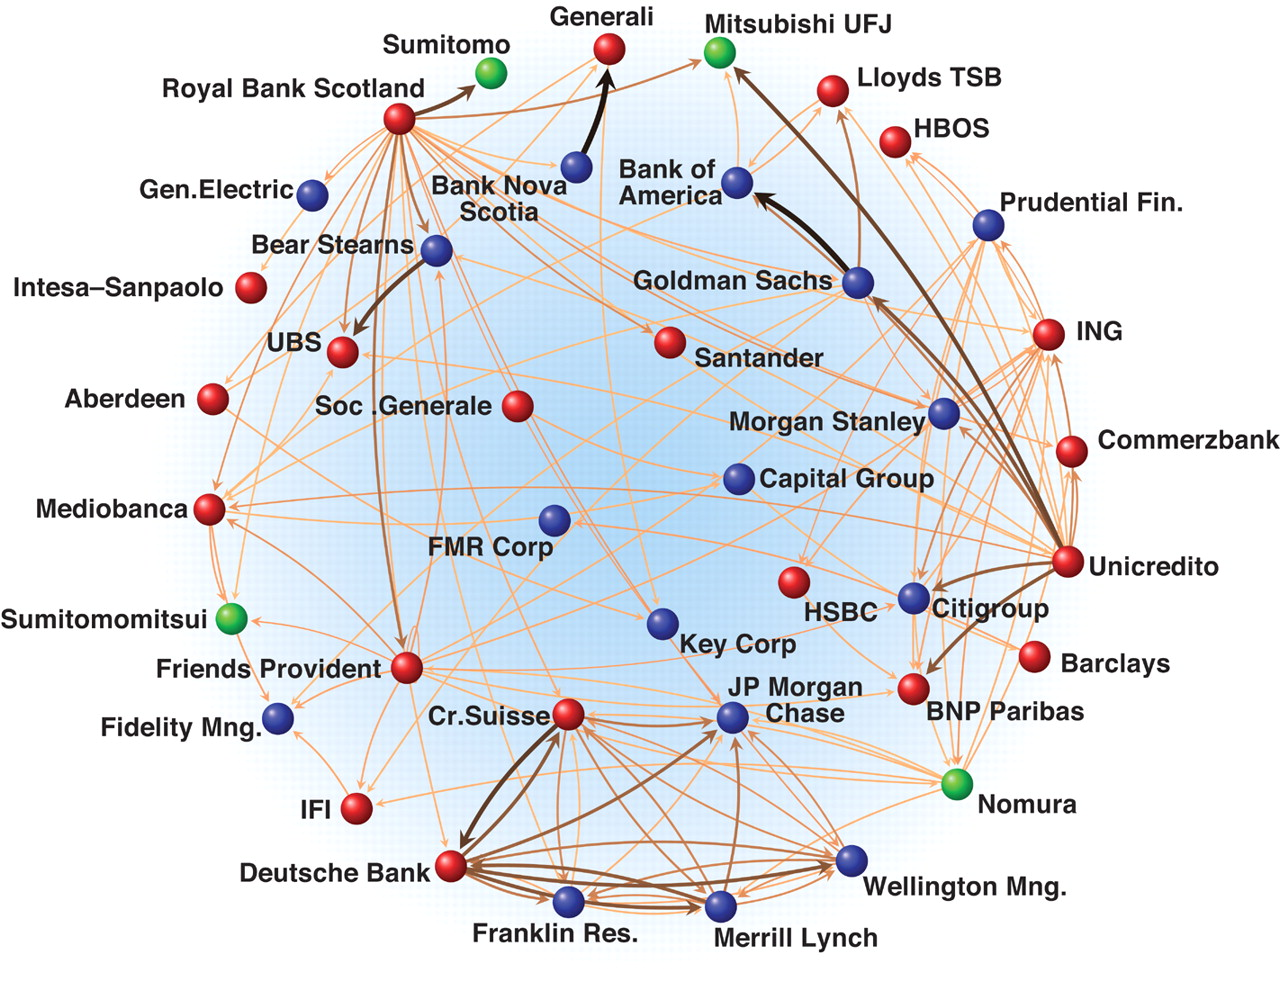
\includegraphics[width=0.5\textwidth]{bank_network.jpg}
		\caption{Bank Network}
		\cite[p. 424]{schweitzer2009economic}
		\label{fig:bank_network}
	\end{figure} 

	\noindent Another interesting application of graphs is to model social 
	interactions. While there are many different areas of interest which make
	use of social connections, the focus of this thesis is placed on gaining 
	customer insights. Indeed, this is one of the main areas where social network 
	companies such as Facebook or search providers like Google make their
	revenue. Those companies mainly generate their revenue by providing customer 
	insights or selling targeted advertising \citep{Facebook2021,Alphabet2021}. 
	Both Facebook and Google have the advantage, that their businesses naturally 
	capture relational or more generally network data. Most researchers and 
	companies however do not have access to such data. Companies for instance 
	may have access to large amounts of customer data. This data however 
	typically does not contain relational information (e.g. which client is 
	connected with which other clients). The same is true for researchers, where 
	social scientists often collect data via anonymous surveys. This makes the 
	collection of network data basically impossible. For that reason, most 
	companies and researchers are limited to working with data such as 
	cross-sectional data that contain no network information. It is important 
	to mention, that there is a lot of network data available online. This 
	network data however typically only contains the network connections. The 
	important feature data such as demographic data, topic specific variables 
	and labels are however typically not available. Without feature data, graphs 
	provide rather limited information for gaining customer insights. 
	This is a data access and data collection problem and is a frustrating 
	reality which also affects this master's thesis. It however motivates the 
	research topic which is presented in section \ref{section:research_topics}. 
	First, a general overview of machine learning is given in the following 
	section.
	
	\section{Overview Machine Learning}

	This section provides a high-level overview of machine learning and
	specifies the type of machine learning task used for this thesis. To
	start, it is important to correctly categorize machine learning. There are
	many related big topics such as data science, big data or artificial
	intelligence and it is often not clear what exactly is meant. An overview
	of how these different terms can be categorized is shown in figure 
	\ref{fig:ml_overview}.

	\begin{figure}[h]
		\centering
		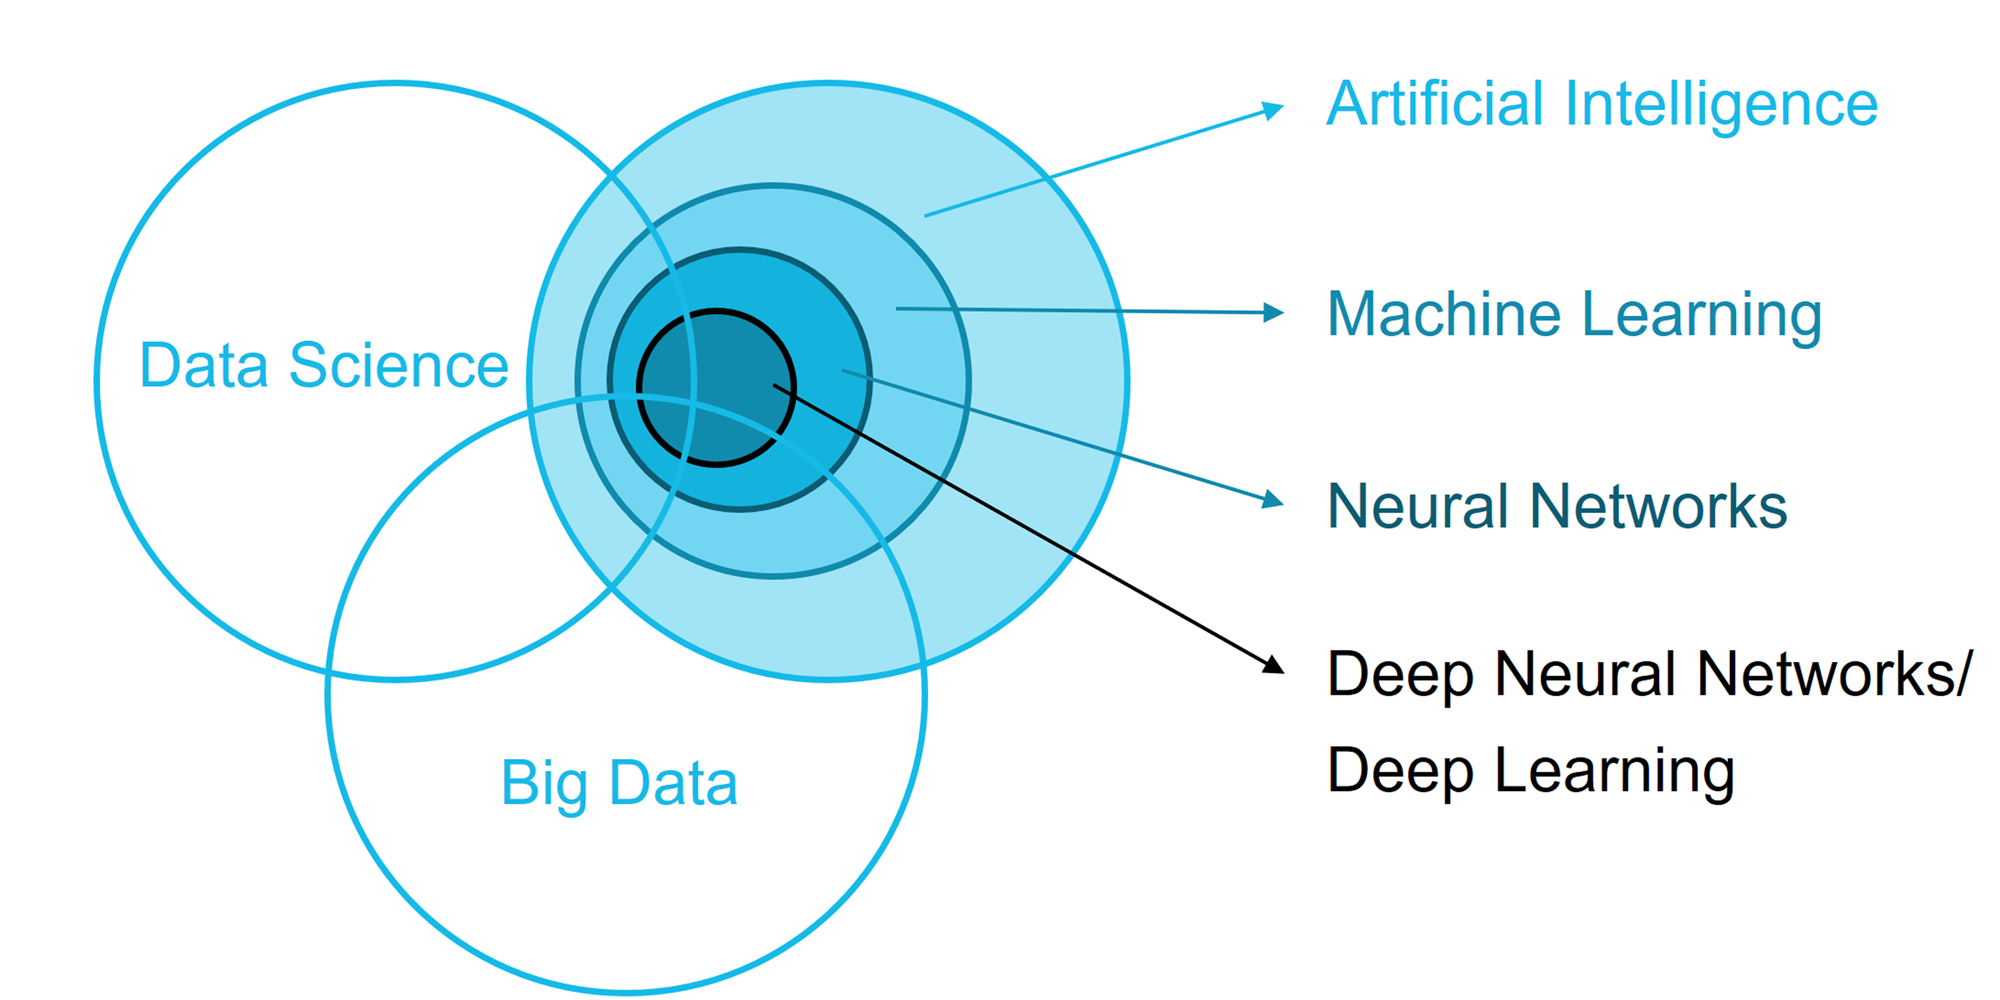
\includegraphics[width=0.7\textwidth]{overview_datascience.png}
		\caption{Overview Machine Learning}
		\citep{Frauenhofer2021}
		\label{fig:ml_overview}
	\end{figure} 

	\noindent Figure \ref{fig:ml_overview} shows well, how these different
	terms are related with each other. Machine learning in particular is
	mostly ascribed to the domain of artificial intelligence. It however also 
	has a shared domain with data science and big data. It is thus at the
	intersection of these three interrelated fields. Machine learning models 
	such as neural networks and deep neural networks are specific models within
	machine learning and are often referred to separately due to their
	popularity. In this thesis, differentiating between machine learning and
	neural networks is not necessary, as the considered machine learning models
	are used for the same task. Machine learning can be applied for various
	tasks and is again best presented visually as shown in figure 
	\ref{fig:ml_tasks}.

	\begin{figure}[h]
		\centering
		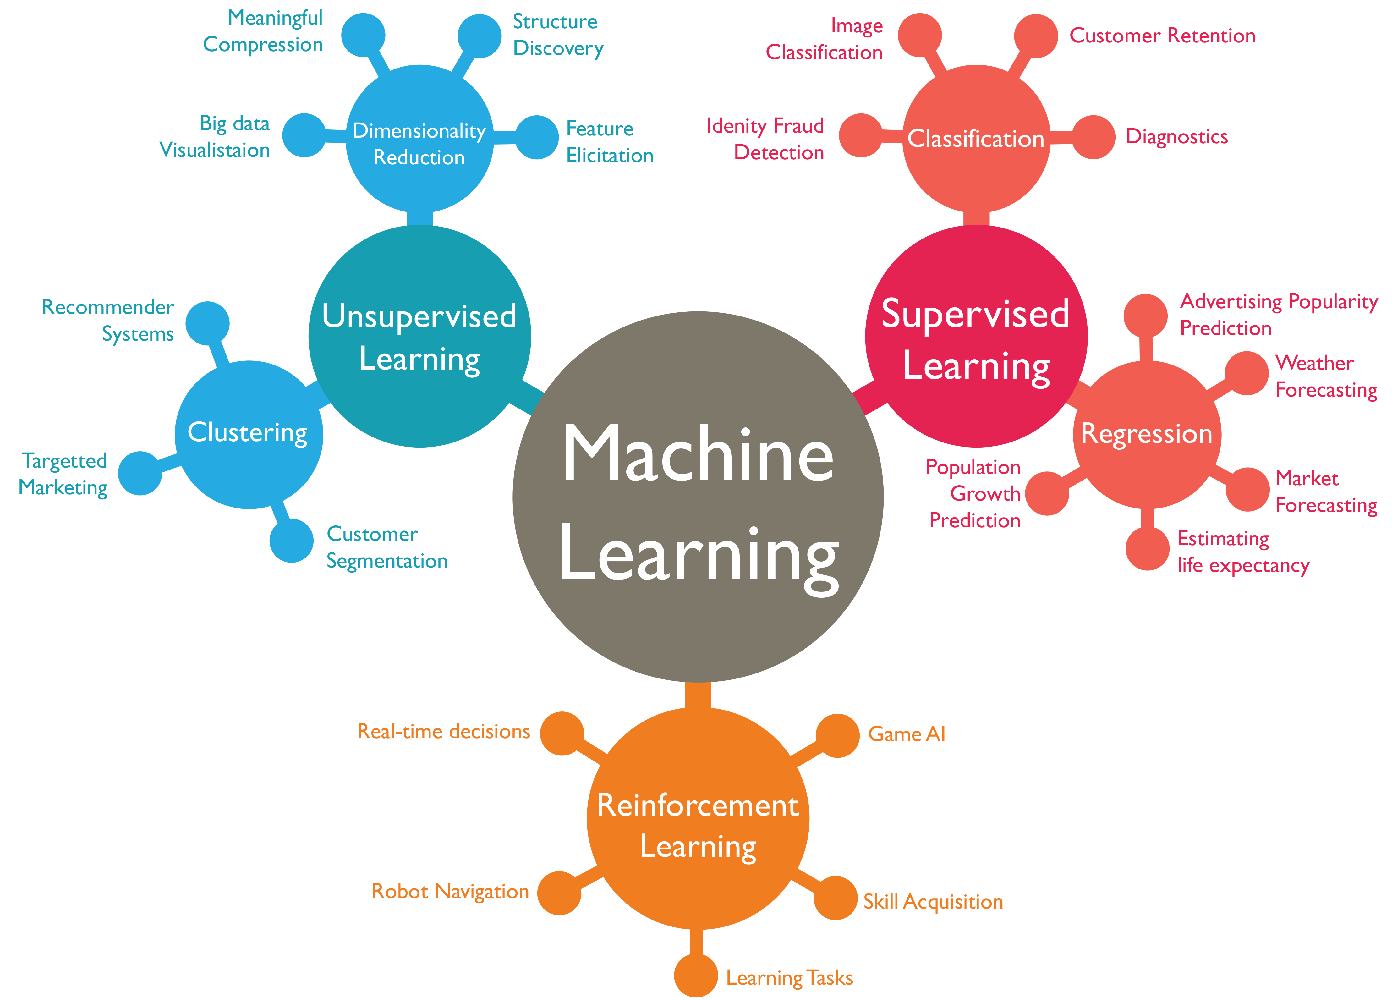
\includegraphics[width=0.8\textwidth]{ml_tasks.png}
		\caption{Overview Machine Learning Tasks}
		\citep{Artisan2020}
		\label{fig:ml_tasks}
	\end{figure} 

	\noindent It is shown in figure \ref{fig:ml_tasks}, that the main tasks for
	machine learning involve classification, regression, reinforcement
	learning, clustering and dimensionality reduction. This thesis focuses on 
	classification tasks. This task is chosen given the available data and 
	because it allows for a nice comparison of different machine learning models. 
	Well known standard machine learning models used for classification tasks 
	include logistic regression \citep{cramer2002origins}, naive bayes 
	\citep{zhang2004bayes}, support vector machines 
	\citep{platt1999probabilistic}, random forest classifiers
	\citep{breiman2001random}, AdaBoost \citep{freund1997decision} and
	artificial neural networks \citep{mcculloch1943logical}. This is an
	incomplete list of popular machine learning models that can be used for
	classification tasks. Popular applications of classification tasks include 
	predicting whether a customer is satisfied, whether to grant a mortgage 
	to a client and many more. The aforementioned machine learning methods have 
	in common, that they all only consider feature data and cannot consider 
	network information. \\

	\noindent Graph machine learning methods are different in that they consider 
	both feature data as well as network information. If one wants to categorize 
	graph machine learning within the framework shown in figure 
	\ref{fig:ml_overview}, it is probably best categorized as a special form of 
	neural network. It is however not a deep neural network, as network depth 
	does not necessarily improve the model and can be even counter-productive. 
	Within graph machine learning, there are two main approaches. The first 
	approach focuses on learning vector representations of graphs which are 
	used for downstream machine learning. The downstream machine learning models 
	include the standard models presented previously. Graph representation 
	learning approaches include models such as DeepWalk 
	\citep{perozzi2014deepwalk} and Node2Vec \citep{grover2016node2vec} among 
	others. The second approach involves the application of graph neural 
	networks for which there exist many different models. These networks 
	include models such as Graph Convolutional Networks \citep{kipf2016semi}, 
	GraphSage \citep{hamilton2017inductive} and many more. \\

	\noindent The detailed theoretical background for the considered graph
	machine learning models is provided in chapter 2.

	\section{Research Topic}
	\label{section:research_topics}

	\noindent The difficult access to graphs which also contain features, 
	motivate the search for alternatives. A review of the literature revealed, 
	that a form of synthetic graph generation could provide a solution to the data 
	access problem. Classic graph generation procedures include the famous 
	Erdös-Rényi graphs \citeyearpar{erdos1959random}, the small-world model by 
	\cite{watts1998collective}, the well-known model by 
	\cite{barabasi1999emergence} and more recently Kronecker Graphs by
	\cite{leskovec2010kronecker}. These models are all very instructive
	regarding the graph generation process and for understanding graph
	properties. These networks however all have the short-coming, that they do 
	not allow for the assignment of feature data to the nodes/observations in the
	network. It became clear, that one has to find or develop a model which 
	makes use of existing feature data for the graph generation process. 
	\cite{kim2012multiplicative} developed the \ac{mag} model. This model makes 
	use of randomly generated feature data which is referred to as attribute data 
	by the authors. The model is shown to be capable of generating random graphs 
	which can adhere to observed real world network properties. An analysis of 
	the \ac{mag} model reveals, that it could also be a useful model for 
	creating semi-synthetic graphs using existing feature data. For that reason, 
	the \ac{mag} model is selected for generating semi-synthetic graphs. This 
	model is introduced in detail in section \ref{section:theory_graphgen}. \\

	\noindent More recently, researchers have focused their attention to
	generative graph models. These models create graphs with features using
	real graphs as a training input. Examples for such models are graph
	\ac{rnn} \citep{you2018graphrnn} and deep generative graph
	models \citep{li2018learning}. These are very fascinating models which can
	be used to recreate or scale graph data. For the purpose of this thesis,
	these models are not purposeful, as it requires an existing graph with
	features to be available. Such a graph is unfortunately not available for
	this thesis. Nevertheless, this is an interesting current topic for graph 
	generation which was considered. \\ 

	\noindent The access problem to graphs which include feature data might be 
	resolved using the \ac{mag} model as previously mentioned. This model is 
	interesting as most researchers and companies have access to large amounts 
	of feature data such as customer databases or survey data. It would be of
	great benefit, if the available feature data could be used for generating
	semi-synthetic graphs. The \acs{mag} model provides a solution for
	generating such graphs. Semi-synthetic graph refers to the fact, that the 
	graph is generated using real feature data. Fully synthetic graphs on the 
	other hand are generated exclusively using artificial data. The goal of the
	semi-synthetic graph is to generate connections between the observations in 
	a given dataset. These connections should enhance the information present
	in the dataset. Graph machine learning should then be capable of exploiting
	these additional connections and hopefully provide competitive if not
	superior results compared to standard machine learning models. This thesis 
	therefore investigates to what extent semi-synthetic graphs can be used for 
	graph machine learning. Of course, semi-synthetic graphs are unlikely to be
	capable of fully substituting the performance of real graphs for machine 
	learning. Nevertheless, semi-synthetic graphs provide additional and 
	hopefully useful network information. To assess these hypotheses, the 
	results using graph machine learning are compared to standard machine 
	learning models. To close this section, the research question as well as the 
	hypotheses of this thesis are presented formally as follows. 

	\paragraph{Research Question}\mbox{}

	\noindent To what extent are semi-synthetic graphs based on real 
				feature data useful for a classification task using machine
				learning?

	\paragraph{Hypotheses}\mbox{}

	\noindent\textbf{H1:} Graph machine learning using semi-synthetic graphs
	provide superior results compared to the results of standard machine
	learning for a given classification task.\\

	\noindent\textbf{H2:} Graph machine learning using semi-synthetic graphs is
	a competitive strategy compared to the results of standard machine
	learning for a given classification task.\\


	\noindent The required theoretical background for this thesis which
	includes graph machine learning, graph generation and graph theory in
	general is provided in chapter 2.
